\section{Simulation Rules} \label{rules}

The simulation runs in discrete steps (\textbf{turns}). The conceptual ``length'' of a turn is
designed to simulate the time to send $k$ bytes, where $k$ is a configurable constant. Each turn, an agent may do any combination of the following: listen, broadcast, move, or die.

\subsection{Movement}

The simulation world consists of a $w$*$h$ grid of signed integers. If a cell's value $c$ is
non-negative, it is the terrain height. Otherwise, the cell is impassable. An agent can move at most
one cell up, down, left, or right per turn. However, after moving into a square, it must wait $c$
turns before it may make another move.

An agent's move may succeed or fail. If an agent tries to move into an impassible cell, it will
fail. It will also fail if it tries to move into a cell that was occupied by another agent at the
end of the last turn, \textbf{or} a cell that another agent attempts to move into in the same turn.
These cases are shown in figure \ref{mvt}.

\begin{figure*}[h!]
    \begin{center}
        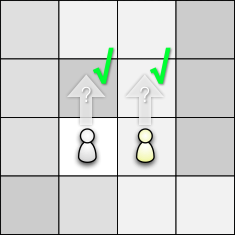
\includegraphics[width=1in]{figures/mvt1.png}
        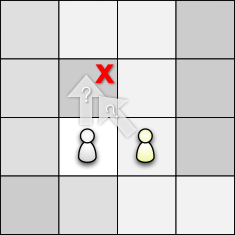
\includegraphics[width=1in]{figures/mvt2.png}
        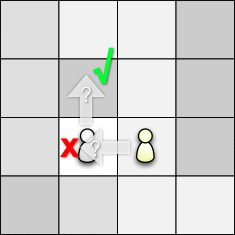
\includegraphics[width=1in]{figures/mvt3.png}
    \end{center}
    \caption{Three main cases for movement.}
    \label{mvt}
\end{figure*}

It may seem more intuitive for both moves in case 3 to succeed, i.e. a move $Z\rightarrow Y$ by $A$
should succeed if agent $B$ moves $X\rightarrow Y$. However, allowing this case would introduce
large dependency graphs that would span a large geographical area. This kind of dependency graph
would greatly reduce the effectiveness of our horizontal scaling scheme based on geographical
partitioning described later in this paper.

\subsection{Messages}

Tecellate simulates radio communication. There are $N$ frequencies an agent can broadcast on or
listen too. An agent may broadcast a fixed number of bytes on a frequency and/or listen on a
frequency. If an agent listens to the same frequency it broadcasts to and no interference is
introduced, the agent will hear its own broadcast at the beginning of the next turn.

\begin{figure*}[h!]
    \begin{center}
        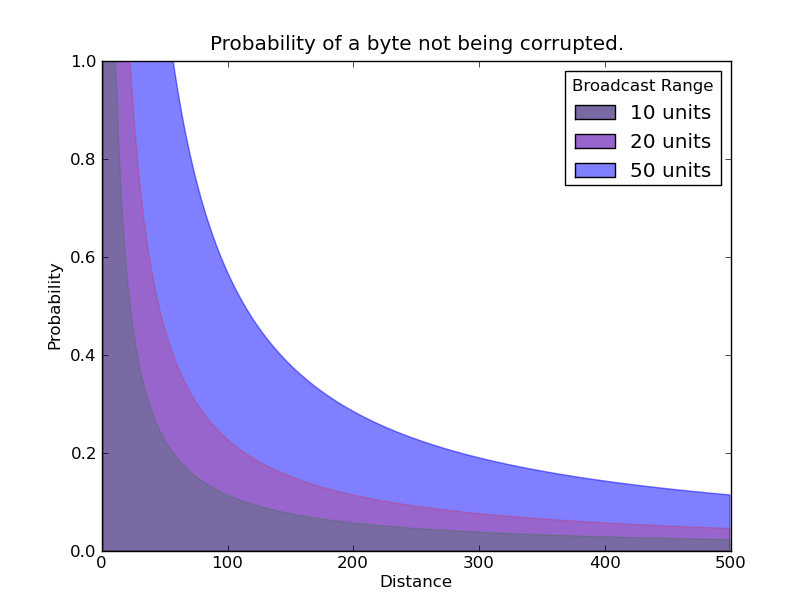
\includegraphics[width=6in]{figures/corrupt.png}
    \end{center}
    \caption{The probability of a byte being corrupted as a function of how far from the receiver
        the byte was broadcast.}
    \label{corrupt}
\end{figure*}

Like radio communication, the messages broadcast decay over distance. When an agent listens to a
frequency, the agent always receives data. However, if no one is broadcasting on that frequency, the
agent will receive random data. Since the message decays over distance, even if an agent hears it,
some parts of the message may be corrupted. The farther away a listener is from a sender, the more
corruption is in the message. As shown in Figure \ref{corrupt}, depending on the strength of the
broadcast, the message is less and less likely to be uncorrupted the farther the receiver is from
the transmitter.

\begin{figure*}[h!]
    \begin{center}
        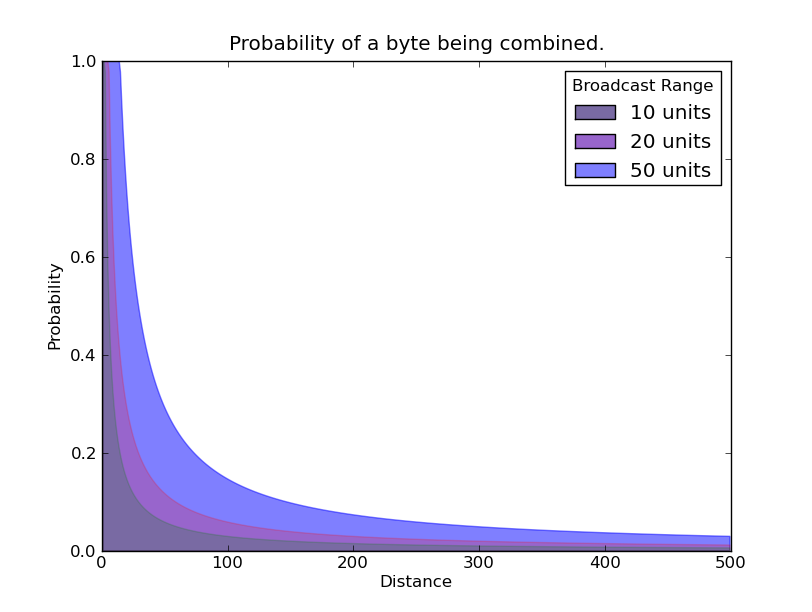
\includegraphics[width=6in]{figures/combine.png}
    \end{center}
    \caption{The probability of a byte being combined into the received message as a function of
        how far from the receiver the byte was broadcast.}
    \label{combine}
\end{figure*}

Corruption of a message can also occur if more than one message is broadcast on the same frequency.
Figure \ref{combine} shows the probability that a byte will be heard by the receiver. If it is heard
it is logically anded with other bytes also heard. Thus, if there are two messages broadcast and the
receiver is close to one of the transmitters but far from the other there is a very low probability
of interference.

\subsection{Energy and Death}

An agent spends 1 unit of energy per turn. If it runs out of energy, it dies. It remains on the
field but cannot take any actions.

Energy gathering has not been implemented but will be an important feature in the future. It was
skipped for this stage of the project because it is simple to implement.

\subsection{Planned Features}

In general, agents are unable to perceive the world. In particular, agents cannot ``see'' terrain or
other agents. We are investigating ways to provide perceptions to agents in a way that match
artificial intelligence expectations well, but felt that the specifics were out of scope for this
project.

As mentioned earlier, energy cannot be gathered, only spent. Agents begin the simulation with fixed
and equal amounts of energy, which makes the energy feature useless in its current state.
